%===============================================================
%%%%%%%%%%%%%%%%%%%%%%%    main.tex   %%%%%%%%%%%%%%%%%%%%%%%%%%
%===============================================================
% All heavy lifting is done in the whitepaper class,
%  stored locally as ./whitepaper.cls
%
% Configuration Options:
%   1. 2-column mode can be *enabled/disabled*; see
%      ./abstract.tex for comments indicating how
%   2. All other configuration settings are defined in our 
%      'whitepaper' document class
%   3. All code listings must use [style=<LANG>] for color
%      output, e.g., \begin{lstlisting}[style=Python]
%===============================================================
%===============================================================
%%%%%%%%%%%%%%%%%        START PREAMBLE        %%%%%%%%%%%%%%%%%
%===============================================================
\documentclass{whitepaper}
\ttl{A Fuzzy Safari}{Adventures in JavaScriptCore Vulnerability Research}
%--------------------------------------------------------------
% Author(s)
\auth{J. Angra}
%\auth{Z. Minneker}
%--------------------------------------------------------------
% Afficiation(s)
\aff{Security Innovation}{}%Boston, Seattle, Pune}
%-------------------------------------------------------------
% Date Stamp
\dtstamp{\today}
%===============================================================
%%%%%%%%%%%%%%%%%%        END PREAMBLE        %%%%%%%%%%%%%%%%%% 
%===============================================================
\begin{document}

% Abstract
% Abstract
\renewcommand{\abstractname}{}
%\twocolumn[\begin{@twocolumnfalse} % COMMENT THIS OUT TO ENABLE SINGLE COLUMN MODE
    \maketitle
    \begin{abstract}
        \vspace{-10ex}
        \centering
        \begin{minipage}{\dimexpr\paperwidth-5cm}
          %------------------------------------------------------------------------
          \ab{
              \textsc{\bf{Abstract.\hspace{1ex}}}%
            \textrm{\noindent Modern browser exploitation has shifted the focus of bug hunting to the browser's JavaScript engine. This component often 
              trends towards high cyclomatic complexity and provides the greatest level of flexibility to a vulnerability researcher. This
              has lead to a variety of bugs in varying subcomponents;  from compiler-, interpreter-, and optimization-based vulnerabilities
              to those triggered from garbage collection, WebAssembly, or the DOM.%
              %Are these vulnerabilities trivial to discover? Are there no more left to discover?%
              %
              We present here, an approach to vulnerability research in modern JavaScript engines. We will primarily focus on \textit{Safari}'s
              internal JavaScript engine, JavaScriptCore. A strong focus on bug discovery, crash identification, and logical reasoning
              provides success and failure over a variety of research approaches, both theoretical and pragmatic. We then outline our
              interpretation on the ideal approach to future work in this relam.%
              %
              %However, the Renderer Process is naturally sandboxed by macOS; the above only makes up Stage 1. Research into general sandbox
              %escapes go back over 20 years, with the first notable exploits performing escapes from the first Java sandbox. Modern
              %research into the Apple Safari sandbox provide detailed and informative resources for us to draw and expand
              %from.
              %
              %A likely path here is Apple's rather bug-full IPC mechanisms, of which there is one major one: Mach ports. They originally were
              %used in the Mach kernel as a way to send messages back and forth from the kernel to various modules, but as XNU, Darwin, and
              %computing as a whole became more complicated, Mach ports became a full back bone for the operating system.
              %However, in their original incarnation, they had no concept of a malicious actor inside the system. Thus, ports run in privileged
              %space, with a security model that has had to be bolted onto them post facto, leading to embarrassing mistakes and a number of
              %vulnerabilities. Other possibilities include macOS's syscall interface, which provides 4 separate styles to perform syscalls
              %in a way that Apple actively discourages developers from using and looking at.
              %%
              %This combination of a large code base (Webkit has ~5 million LOC), a continuously changing modular architecture, and thorough
              %detailed analyses from renowned researchers provides us a fruitful target to develop and hone our research methodologies and skills
              %in the Darwin environment.
            } 
          }
          \keywords{Keywords: javascript, fuzzing, intermediate representation, speculative reasoning}%
          %------------------------------------------------------------------------
          % Journal Edition 
          % \DOI{\urlstyle{same} \url{https:/doi.org/xxxxxxxx}    \hspace{8.5cm}    ISSN 1850-1168 (online)}
          %------------------------------------------------------------------------
        \end{minipage}
        \vspace{7ex}
    \end{abstract}
%\end{@twocolumnfalse}]  % COMMENT THIS OUT TO ENABLE SINGLE COLUMN MODE


% Contact Info (displayed in footnote)
\email{
  %research@bynx.io \\ 
  %PGP:\textsc{91e958db0cc8a0e0adbf4df9d79f1ecb60e882f2}
}  

% No page numbers on first page
\thispagestyle{empty}
\pagenumbering{arabic}
\setcounter{page}{1}
%\newpage

% Display page numbers and current section in header for every page after first
\pagestyle{headings}

% Sections
% 1. Background
%   1.1. Browser Software
%     1.1.1 Process Architecture
%   1.2. JavaScript Engines (high-level breakdown of core components)
%     1.2.1. Parser & Bytecode Compiler 
%     1.2.2. Interpreter
%     1.2.3. JIT Compiler
%     1.2.4. Garbage Collector
%===============================================================
\section{Background}
\setcounter{section}{1}

%===============================================================
% Background on Browsers
%===============================================================
\subsection{Browsers}
In the thirty years since \textit{WorldWideWeb}\cite{berners-lee_www}, the first web browser,
the architecture of the \textsc{World Wide Web (Web)}, and thus web browsers, has exponentionally grown
in both complexity and use. Global strives in consumer technology have allowed billions\cite{browser-stats-world} of users to
access the \textsc{Web}, often through a web browser. Naturally static HTML pages were insufficient;
users wanted \textit{interactive} pages, custom page styling, support for additional media types,
and interconnectivity between two or more \textsc{Web} resources. Today, the \textsc{Web} still
uses HTML, but it's architectural tours de force is the JavaScript language\protect\footnotemark.
\footnotetext{Amoung numerous others, e.g.: PHP, WASM, Go-lang, CSS, etc.}%

\noindent
Modern browsers are built on layed components, running at least two processes: (1) A
primary (main) browser process, for the application itself, and (2) one or more renderer
process. An example architectual diagram is provided as \textit{Figure 1}.%
% Browser Components %
\begin{figure}[!h]
    \begin{center}
        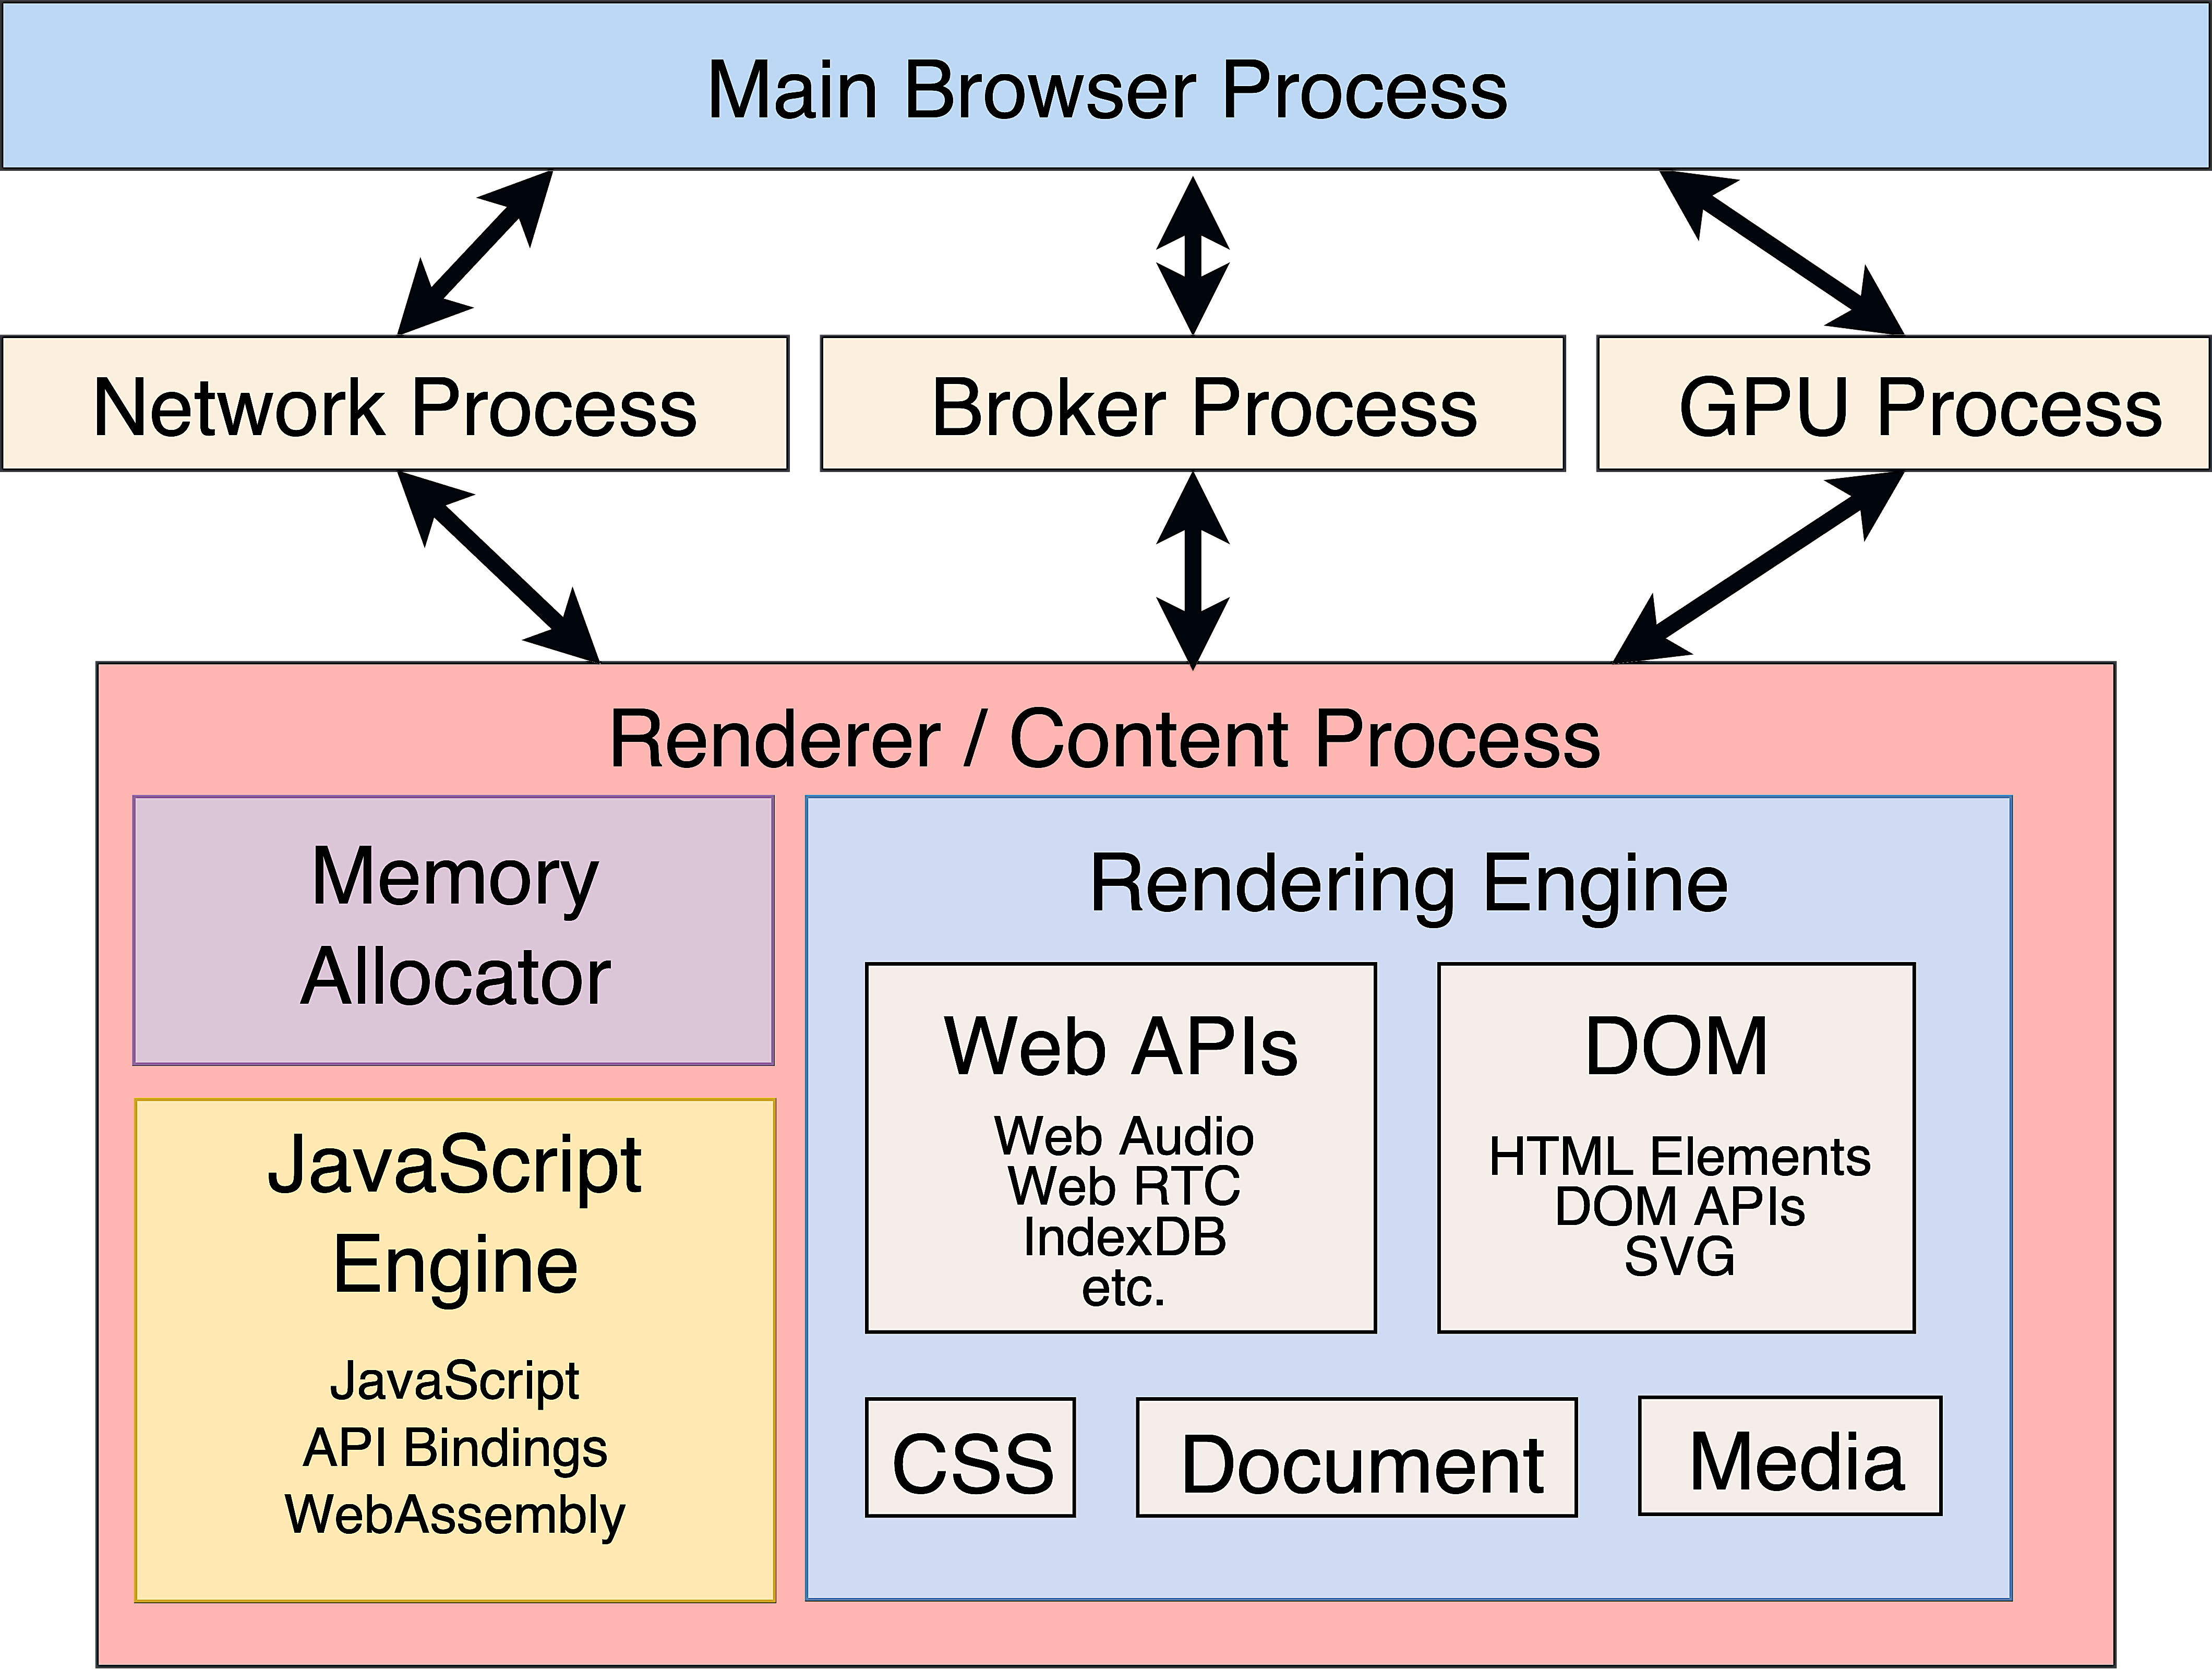
\includegraphics[width=0.475\textwidth]{./img/browser-process-architecture}
        \caption{Process achitecture of a modern web browser.}
    \end{center}
    \vspace{-4ex}
\end{figure}

%% Definition: \newcommand{\p}[1]{\paragraph{\itseries\scshape{#1}}}
\p{Main Browser Process }%
This process is the primary controller for all computaiton; it displays the user interaface and
manages the all processes. Safari, specifically, utilizes a split-process model\cite{wk2}, where
each tab's web content lives in a seperate, isolated, renderer (web) process, spawned per tab.
Although this model improves stability and performance, it's greatest significance is this model
also provides the basis for a sandboxing infrastructure; ideally one that will limit damage
to the system, if a rederer process is compromised.

\p{Renderer Process. }%
This component parses \textsc{HTML}, \textsc{CSS}, \textsc{JS}, numerous image/video formats,
and any other varing data formats required to construct the document.
In additional to the core language features, numerous browser APIs allow
developers to interact with this document, or rather Document Object Model
(DOM), retreive data over the network, access web databases, and
more $-$  all via JavaScript. \\
% WebKit Component Boundaries %
% TODO: Remove this if no longer needed
%\begin{figure}
%    \begin{center}
%        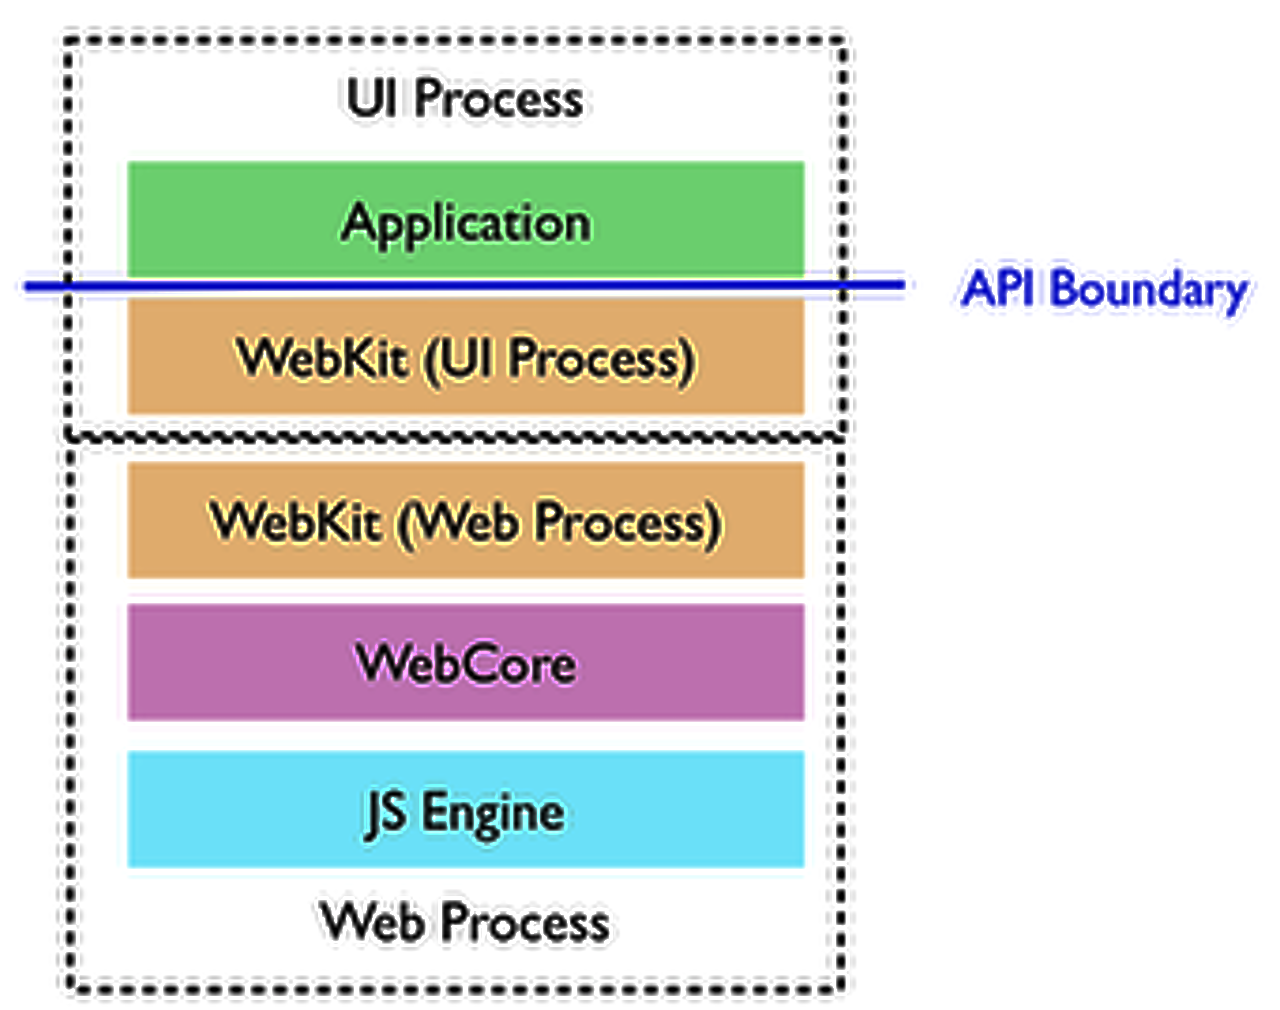
\includegraphics[width=0.475\textwidth]{img/inv}
%    \end{center}
%    \caption{WebKit Process Model}\vspace{-5ex}
%\end{figure}

From a security standpoint, the renderer retreives, lexes, parses, compiles [to C++], and
displays a multitude of untrusted and potentially complex JavaScript inputs; it is the most
exposed browser component. As such, it's commonly sandboxed\protect\footnotemark, limiting
access to sensitive data and applications, both internally and within the device's operating
system or underlying kernel.
\footnotetext{The complements of this paper's work can found here <link to zach's paper/stuff>}

%===============================================================
% Background on JS engines and JavsScriptCore
%===============================================================
\subsection{JavaScript Engines}
JavaScript, a weakly-typed scripting language, is one of the largest components of modern websites.
Naturally, the need for high performance script exectuion resulted in deeply complex engine
implementations; the perfect place to hunt for complex, domain-specific vulnerabilities. Modern
JavaScript engine typically consist of a runtime and the following components:

\p{Parser and Bytecode Compiler. }%
The parser and bytecode compiler are responsible for converting JavaScript source
code to an engine-specific bytecode representation, for use by the interpreter and JIT
compiler. Parsing tokenizes the input stream and contructs an Abstract Syntax Tree (AST)
based on grammartical sytax of JavaScript. The AST is subsequently compiled to bytecode.%
%(i) a parser and bytecode compiler, (ii) an interpreter for aforementioned bytecode,
%(iii) at least one Just-in-Time (JIT) compiler, (iv) and a memory allocation mamangement system, a Garbage Collector (GC).
%
%
% integrate bytecode example better %
\begin{lstfloat}
\begin{lstlisting}[style=JS,caption=Example function to JIT compiler]
// add.js
function add(a,b) {
    return a + b;
}
add(2, 1337);
\end{lstlisting}
\end{lstfloat}
%
\vspace{-1.5em}\noindent
The bytecode is the source of truth throughout the whole engine. While some engines, such as
Spidermonkey, use a stack-based virtual machine, other engines, e.g., JavaScriptCore, use a register-based
virtual machine. As such, their bytecode format is fundamentally different. However, one typically common
shared property is that bytecode is untyped: the bytecode operates on weakly-typed values which
contain both type- and value-information. During execution, an interpreter will perform
different actions depending on the runtime type of the operands.
%
\begin{lstfloat}
\begin{lstlisting}[style=asm, caption=Interpreter bytecode and type profile]
// jsc -d add.js
bb#1
[   0] enter
[   1] get_scope    dst:loc4
[   3] mov          dst:loc5, src:loc4
[   6] check_traps
[   7] add          dst:loc6, lhs:arg1, rhs:arg2, operandTypes:OperandTypes(126, 126)
[  13] ret          value:loc6
\end{lstlisting}
\end{lstfloat}
%
\vspace{-1.5em}\noindent
Another property common to the resulting bytecode is that it is usually unoptimized. This is primarily done
for two reason: (1) To keep the overall startup time as low as possible, forbidding the use of costly
optimizations, and (2) many optimizations require type information, which is not available at this point,
due to the weakly-typed nature of the language itself.
%
\p{Interpreter. }%
The task of an interpreter is to consume the bytecode and execute it. As the bytecode is specific to
a given engine, so id the interpreter. Interpretation happens by fetching the next bytecode instruction
from the currently executing code and dispatching it to the handler for the bytecode operation.

\noindent
While interpretation of bytecode is fairly slow, in part due to the unoptimized nature of the bytecode
and high dispatching overhead, the initial startup time is minimal. Thus, for simple or sparsly repeated
operations it's overall better to execute it directly via the interpreter; the overhead compilation
would introduce simply outweighs the faster execution speed of the resulting machine code. Conversely,
if code segment/block is repeatedly executed by the application it is worth optimizing that code. This is
the job of a JIT compiler. As current JIT compilers usually require type hints to produce optimized machine
code, it's also the job of the interpreter to collect type profiles during bytecode execution. Often this
is performed by augmenting the bytecode with previously seen input types for each bytecode operation. An
example of bytecode after it has gone through this process in JavaScript core is provided in 
\textit{Listing 3}, below.
% JSC takes this even further, 'typed' bytecode is interpretted and used to perform speculative optimization %
% (^) footnote or section? %

%===============================================================
% JSC Bytecode interpreter
% JSC specifics on bytecode and register typing %
%   Not sure where to put this, yet - if at all %
%With the new infrastructure, when declaring an instruction, a name and type must be given for each
%of the operands, as well as declaring all the data that will be stored in the metadata table.
%
\begin{lstfloat}
\begin{lstlisting}[style=JS,caption=JavScriptCore SyntaxType for OpAdd]
op:add,
  args: {
    dst: VirtualRegister,
    lhs: VirtualRegister,
    rhs: VirtualRegister,
    operandTypes: OperandTypes,
  },
  metadata: {
    arithProfile: ArithProfile,
  }
\end{lstlisting}
\end{lstfloat}%
\vspace{-2.5em}%
%With this extra information, it is now possible to generate a fully typed struct for each instruction:
%
%\begin{lstfloat}
%\begin{lstlisting}[style=JSC++,caption=JavScriptCore Syntax Type for OpAdd]
%SLOW_PATH_DECL(slow_path_add)
%{
%   OpAdd bytecode = pc->as<OpAdd>();
%   JSValue lhs = GET_C(bytecode.m_lhs);
%   JSValue rhs = GET_C(bytecode.m_rhs);
%   ...
%}
%\end{lstlisting}
%\end{lstfloat}
%
%In the example above, we first need to convert the generic \textsc{Instruction* pc} to the instruction we
%want to access, which will perform a runtime check. If the opcode matches, it returns an instance
%of the generated struct, OpAdd, which includes the fields \textbf{m\_lhs} and \textbf{m\_rhs}, both of type VirtualRegister as specified in our instruction declaration.
%===============================================================
%
%
\p{JIT Compiler. }%
A JIT compiler acts as an alternative to an interpreter for script execution. It, too,
consumes bytecode by the parser, as well as type profiles gathered during execution by the
interpreter.  Having access to both, it converts the bytecode to optimized machine code which
can be executed directly on the host CPU.%

\noindent
As JIT compilers are crucial to execution performance, they are the subject of intensive research.
Many implementations and key mechanisms have been discussed, e.g., polymorphic inline
caches\protect\footnotemark.
\footnotetext{Polymorphic Inline Caching is a broadly used mechanism to speed up polymorphic
operations in dynamic language interpreters and at the same time gather type information
for the JIT compiler by caching results of previous executions.}

\noindent
A JIT compiler will often, initially, convert the bytecode to another custom intermediate representation.
This IR is often graph based to facilitate the various optimizations that are later performed on it. In
addition, most engines currently use a static single assignment (SSA) form to further simplify code
analysis and optimization; JavaScriptCore utilizes a two-tier IR consisting of Bare Bones IR and AIR.%
% code snip examples? %

\subparagraph{\textit{Speculative Optimization. }}%
% we focus on the JIT compilers: DFG,FTL
% go through DFG vuln example
One essential mechanism that allows generation of performant machine code for JavaScript
and dynamically typed languages, in general, is speculations: equipped with type profiles from the
interpreter, the compiler \textit{speculates} that the same types will be used in the future. It will
then guard these assumptions with runtime guards: small fragments of code that perform an inexpensive
type check and bailout if the check fails, in which case execution will continue in a more generic
execution tier, i.e., the interpreter. These type-guards essentially convert the previously untyped
code into strictly typed code, which may subsequently be optimized in a similar fashion as other
strictly-typed languages, such as C++ or Java. This mechanism is shown in \textit{Listing 4} using an
imaginary bytecode and compiler IR format.

\begin{lstfloat}
\begin{lstlisting}[style=JS,caption=Compiler IR for interpreter bytecode\protect\footnotemark]
function add:
  v0 = LoadArgument 0  
  CheckIsInteger v0

  v1 = LoadArgument 1  
  CheckIsInteger v1
    
  v2 = IntegerAdd v0, v1
  Return v2
\end{lstlisting}
\end{lstfloat}
\footnotetext{Type profiles were used to emit type checks and optimiatize specialized integer addition instructions.}

\vspace{-1.5em}\noindent
It is not uncommon for an engine to have multiple levels of JIT compilers.  These correspond to
different optimization levels: the early JIT compilers perform less optimizations, thereby produce
machine code faster. The late JIT compiler stages perform more optimizations,thereby generating
faster machine code.  A unit of code may be recompiled by a higher level JIT compiler when its
execution count reaches another threshold.  JavaScriptCore, the engine inside WebKit currently
features three different JIT compilers in addition to an interpreter. V8, the engine inside the
Chrome browser, on the other hand, only uses one JIT compiler and one interpreter.%

\begin{figure*}[!t]
\begin{center}
    \vspace{-5em}
    \begin{minipage}{\dimexpr\paperwidth}
    %\def\svgwidth{584bp}
    \def\svgwidth{\paperwidth}
    \scalebox{0.85}{\input{./img/optimization-workflow-c-vs-js.pdf_tex}}\vspace{-2em}
    \end{minipage}
\end{center}
\caption{JSC Speculative Optimization WorkFlow}
\end{figure*}

\noindent
Here, the function to be compiled, which is shown in \textit{Listing 1} is invoked with integers as arguments. This is
captured by the interpreter in-type profiles associated with the bytecode as shown in \textit{Listing 2}.
Based on those, the JIT compiler speculates that the same types will be used in the future and guards
that assumption with two type checks. Afterwards, the compiler can use fast, specific operations, such
as the addition of two integers, in lieu of slow, generic ones that cover all possible scenarios of
different types. This can be seen in \textit{Listing 3}. The integer addition used in this example could well
be implemented with a single machine instruction instead of the generic addition operation as defined
by the language specification.%
% TODO: Add img/ftl_pipeline.png somewhere %

\p{Garbage Collection. }%
As JavaScript frees the programmer of the responsibility to return allocated memory back
to the system, it requires a garbage collector (GC) to detect and reclaim unused memory.%

\noindent
Most high-performance garbage collector systems are based on the mark-and-sweep algorithm, which
operates in two phases. First, during the periodic marking phases, the whole graph of reachable
objects is scanned. Then, during the sweeping phase, every memory allocation which was not visited,
implying that it is a dead object, is freed and returned to the allocator.%

\noindent
Various extensions of this core algorithm exist and are in use today. One key improvement lies
in concurrent marking to avoid noticeable pauses in the application caused by ”stop-the-world”
garbage collection. Modern collectors such as \textsc{Riptide}\protect\footnotemark, the collector used in
JavaScriptCore, further strive for a minimal amount of application interrupts due to garbage
collection through parallelism, if multiple CPU cores are available.
\footnotetext{\textsc{Riptide}, was not targeted for this research.}

%===============================================================

\newpage
% 2. Motivation 
%   2.1. State of Fuzzing
%   2.2 JSC Speculation
%   2.3 WebAssembly
%===============================================================
\section{Motivation}

\subsection{State of World}

The fundamental challenge of JS engine fuzzing can be summed up by the observation that,
while we know the comeplte source and specification of our target source and exploitation language, respectively,
the number of degrees of freedom in such an envrionment is much too large to allow for a direct, instantaneous
identification of all vulnerabilities. This observation is reflected in the multitude of architectures and
approaches in today's JS engine fuzzers.

The space of today's JavaScript engine fuzzers can best be understood
as two mutually non-exclusive architectures: generative and mutational.
\vspace{-1em}%

\p{Generative fuzzers} posit new test cases 
(i) from scratch based on a predefined grammar, e.g., DOMato\cite{domato} and Dharama\cite{dharma}, or
(ii) by constructing them from synthesizable code blocks, e.g., CodeAlchemist\cite{codealchemist_2019} and Fuzzilli\cite{saelo_thesis}.

\p{Mutational fuzzers} posit new test cases using segments either learned from seed-based mutations
or borrowed from other corpora programs, e.g., Skyfire\cite{skyfire_2017}, Fuzzilli\cite{saelo_thesis},
Nautilus\cite{nautilus_2019}, Superion\cite{superion_2019}, and DIE\cite{die_2020}.

%-----------------------------------------
\subsection{JSC Speculative Type [Confusion]}

%<Short paragraph on the focus of JIT compilers and type speculation>
One of the more prominant observed vulnerabilty classes, type confusion vulnerabilities often require a complex 
control and/or data flow within the phases of an optimization pipeline. During a given optimization phase,
JavaScript code is profiled, variable types are speculated, and optimized bytecode is produced\footnotemark.
\footnotetext{Poor type speculation results in execution a priori; JSC defaults to unoptimized interpreter bytecode execution.}
A side-by-side view of JSC's speculative optimzation workflow and a standard C-based compiler's equivalent is
provided in Figure 2.

%As we've seen, there are too many components of the JS engine to cover -- following recent exploitation trends,
%we will focus our time (and this paper) on JavaScriptCore's two most attacked components: the \textbf{Data Flow Graph (DFG)}
%and \textbf{Faster Than Light (FTL)} JIT compiler.%

%<we attack these such that we can focus on attacking type speculation, ideally looking for OOB RW>
\begin{itemize}
  \item One of the goals of DFG is to optimize away redundant operations such as type checks
  \item Only a few operations can alter an object’s type
  \item If no such operation is encountered, it can be
  assumed that the object type will stay unchanged
  and a single type check will suffice to prove the type
  of a specific value until some potentially dangerous
  operation is encountered
  \item Operations which may invoke arbitrary JavaScript are dangerous
  \item The arbitrary JavaScript may execute any operation, including things that may mutate an object’s type
  \item Important to model which operations may or may not do this in order to invalidate previously proven types
  \item We may cause arbitrary type confusions by mutating object types
\end{itemize}


%A high-level perspective of this compilation pipeline is presented in \textit{Figure 3}
%\begin{figure}[h]
%  \begin{center}
%    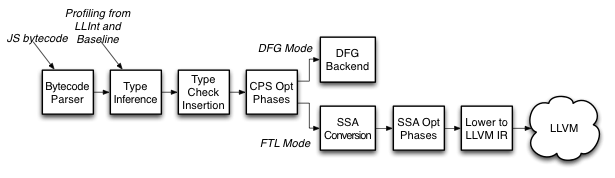
\includegraphics[width=0.5\textwidth]{img/ftl-pipeline}
%    \caption{The JavaScriptCore DFG/FTL JIT pipeline.}
%  \end{center}
%\end{figure}\vspace{-1.5em}

%-----------------------------------------
\subsection{WebAssembly}


\begin{itemize}
    \item WASM growing in popularity, in general
    \item Research into WASM-based fuzzing of JS engines underway, but not much novel research published
        %<opportunistic looking state of it's current research (no one is really fuzzing this)>
    \item WASM code is not JIT'd, thus it utilizes a different pipeline for execution, one that will not affect out primary research
\end{itemize}
%


% 3. Methodology 
%   3.1. Improving Implementation
%     3.1.1. Speeding up Fuzzilli via Inter-Process Communication (IPC)
%     3.1.2. Speeding up Fuzzilli via Inter-Process Fuzzing (IPF)
%     3.1.3. Collective IPF
%   3.2. Extended Code Generation: WASM
%     3.2.1. Constructors
%       WebAssembly.Global
%       WebAssembly.Module
%       WebAssembly.Memory
%       WebAssembly.Instance
%       WebAssembly.Table
%     3.2.2. Static Methods
%       WebAssembly.instantiate()
%       WebAssembly.instantiateStreaming()
%       WebAssembly.compile()
%       WebAssembly.compileStreaming()
%   3.3. Streamlining Triage
%     Linux => ASAN macOS => ASAN 'latest' macOS
\section{Methodology}
Rather than build a fuzzer from re-hashed ideas, the work presented in this paper expands the work of Samuel Gro{\ss}'s \textit{Fuzzilli}.

\subsection{Improving Our Intrumentation}

Fuzzilli's execution model critically relies on Swift's RunLoop Scheduling interface\cite{apple_dev_doc}.
RunLoop's provide developers a programmatic interface to objects of an \textit{input source}; for our work, input sources take the form of an event queue. Thus,
the fuzzing process defaults to corpora sample execution, only diverging for \textit{observered} events whitnessed in the RunLoop event queue.

To take complete advantage of our hardware, Fuzzilli includes an inter-machine communication module, synchronizing instances
over a simple TCP-based protocol. This design allows the fuzzer to scale to many cores on a single machine as well as to many
different machines. One particularly important caveat: TCP synchronization introduced a (fairly sizeable) execution bottleneck. As a result,
three alternative synchronization and one alternative instrumentation models were introduced and tested:\vspace{-1em}

\p{Native IPC} Unix Domain sockets with great deal of shared memory was tested first.
Swift does not like IPC \textit{unless it uses Mach ports}
we were working completely in a debian-based linux distro
\vspace{-1em}

\p{Container-Isolated IPC} Portability, amoung effeciency, are of vital importantce; we simply isolates the
fuzzing system using Docker.

Overhead of Docker was negligible relative to the aforementioned IPC architecture.
\vspace{-1em}

\p{Inter-Process Collective Communication (IPCC)} Inspried by HPC execution models, the C-based OpenMPI
\textit{scatter} and \textit{reduce} functions were used for corpora distribution and sychronization, respectively.

A visual representation of the \textit{Scatter-Reduce-Repeat} collective communication model is provided in Figure 3.
All fuzzing nodes share corpora slices with each other, deduplicating and synchronizing samples in real-time, at regular intervals.

\begin{figure}[!h]
    \begin{center}
        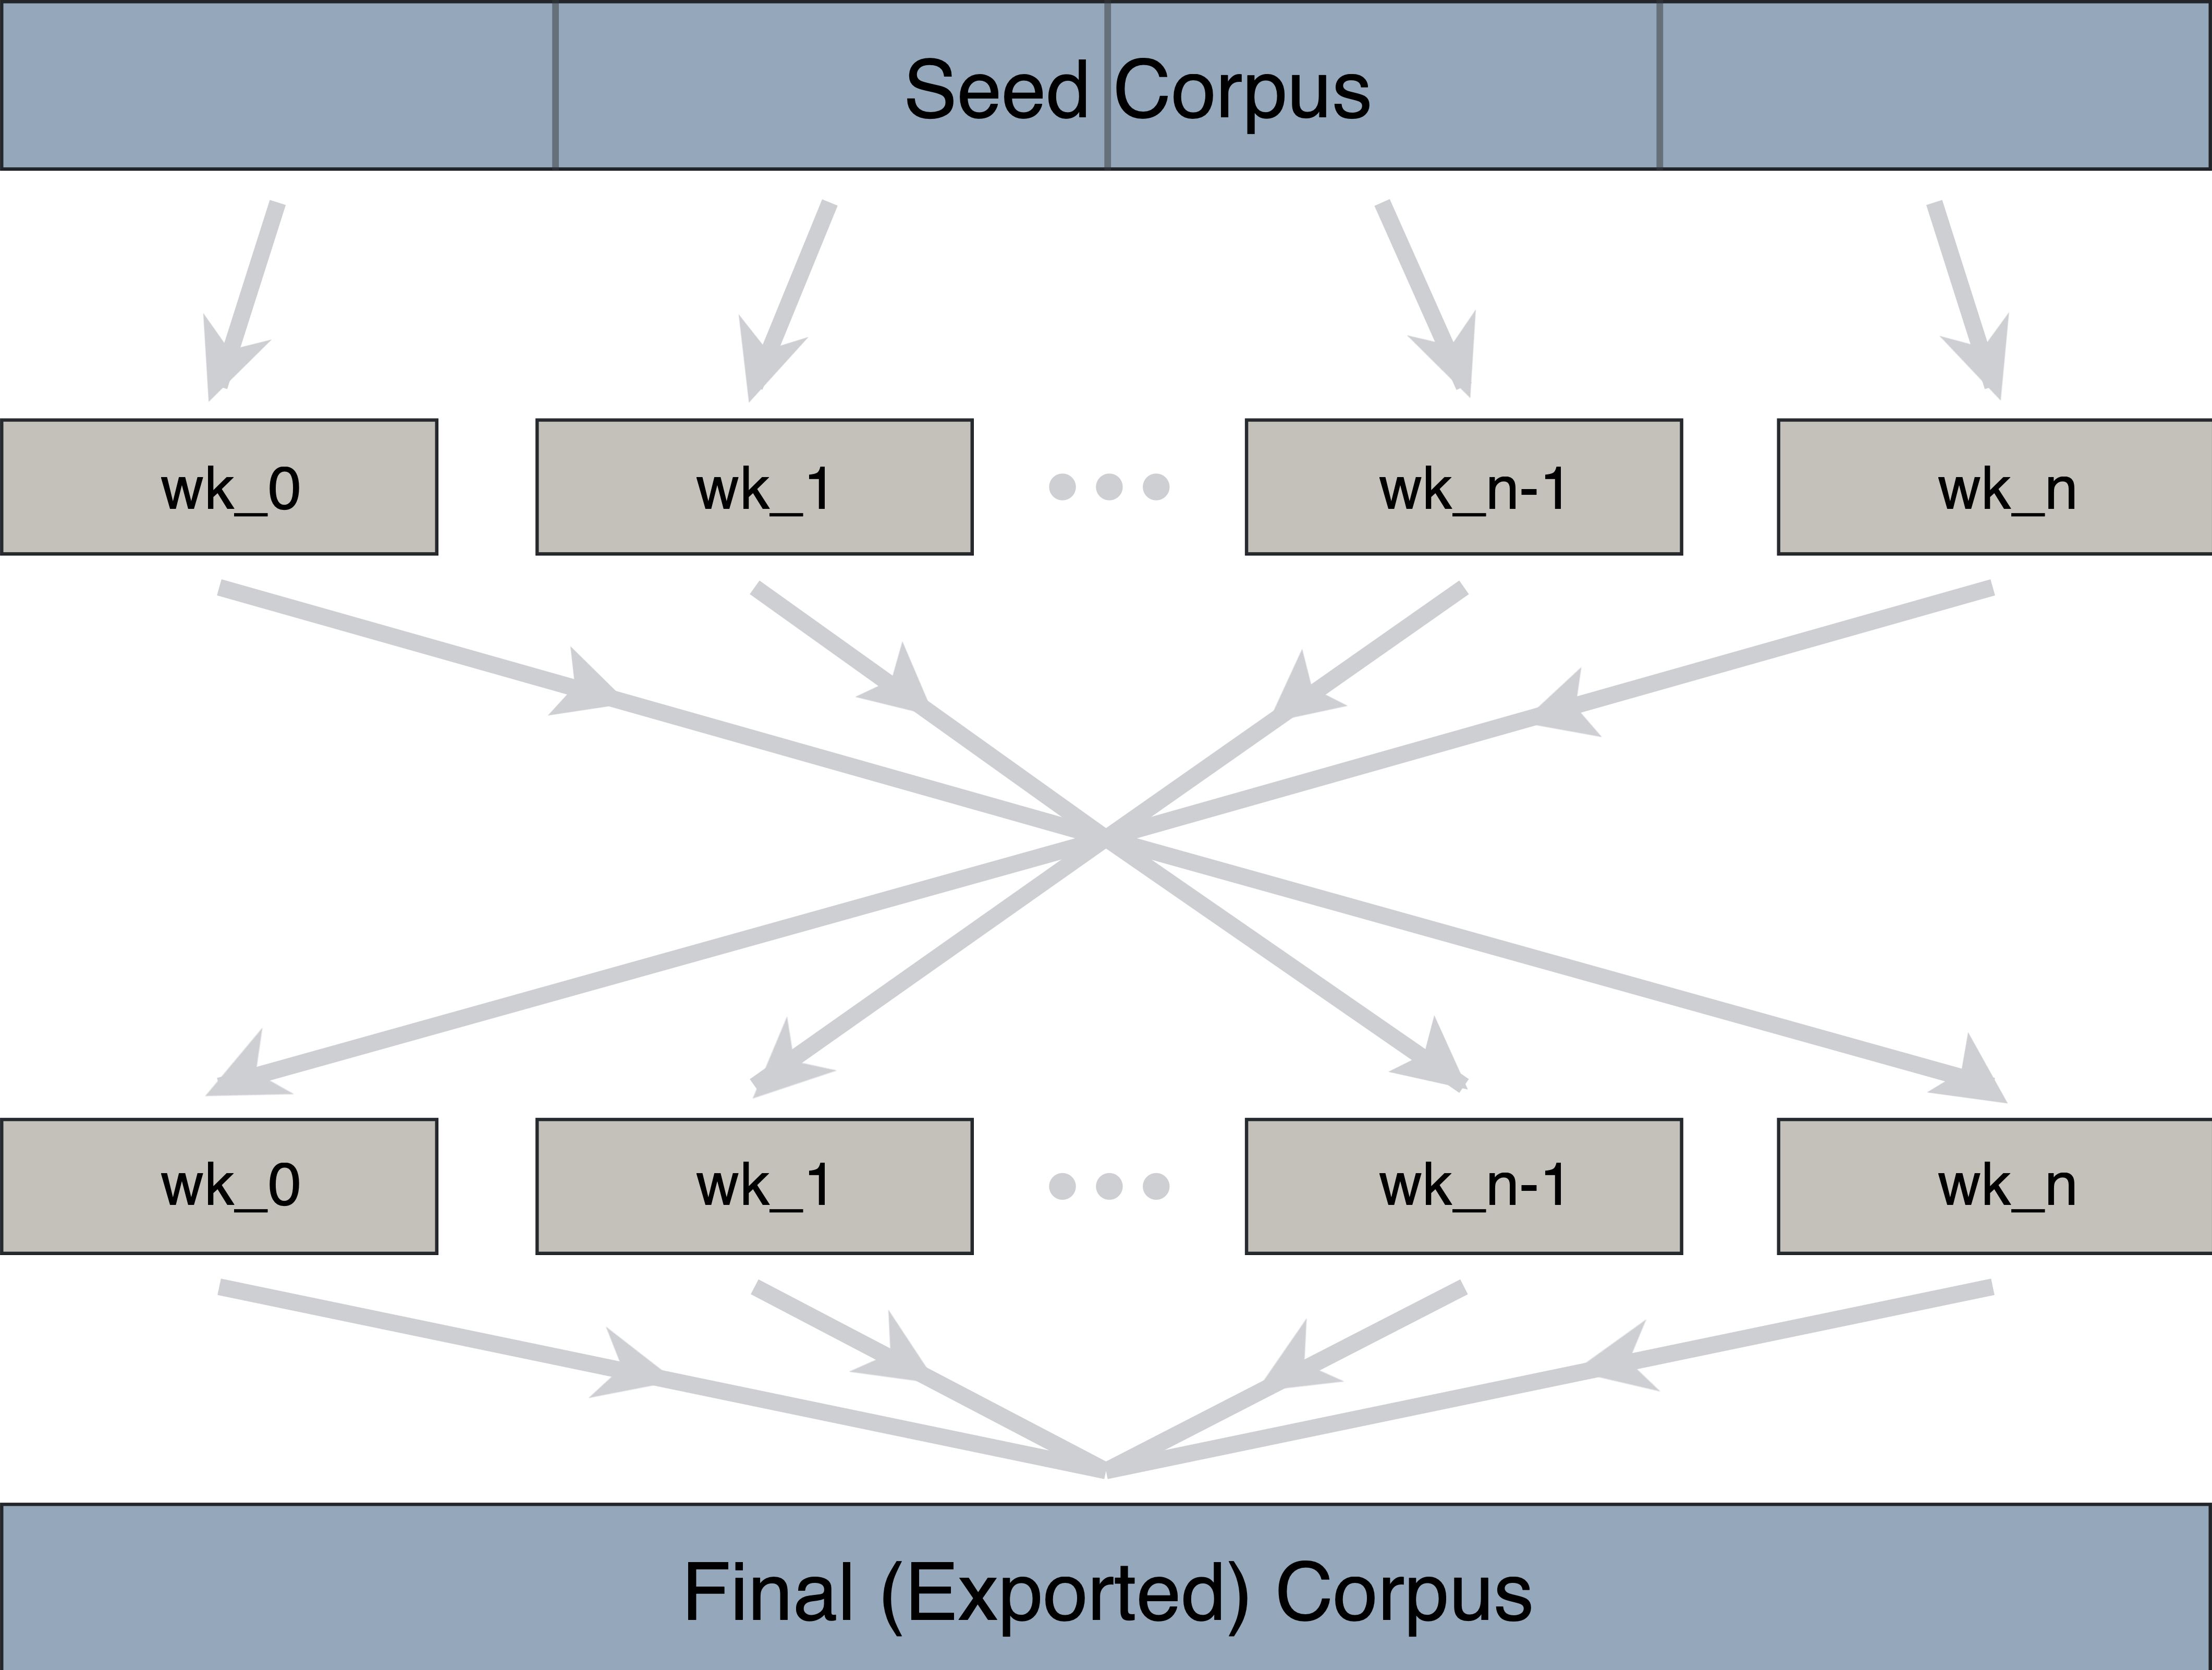
\includegraphics[width=0.45\textwidth]{./img/fuzzilli-topology}
        \caption{Scatter-Reduce-Repeat MPI fuzzing topology. Each cycle, N-equipartitions of
        the seed corpus are ingested by N fuzzing nodes, which operate for some time, then
        corpora slices concatenate and deduplicate into a single corpus.}
    \end{center}
\end{figure}\vspace{-1em}

\p{Skipping The Parser} The primary components of focus for this work are JSC's JIT compilers -- do we really need
to fuzzing the \textit{entire execution pipeline}? JS engine vulnerabilities often require a complex execution flow to trigger a
crash; fuzzing the entire pipeline ensures that we \textit{can} reach all components. Furthermore, only syntatically valid samples
make it past JSC's LLInt.

If we can assert the syntatic validity of our samples, LLInt could be skipped, effectively resulting into direct fuzzing
of \textsc{libJavaScriptCore}. Thus, we hypothesize that such an architecture would greatly improve execution speeds and results.
To test such a hypothesis Rust Foreign-Function Interfaces (FFIs) into \textsc{libJavaScriptCore} native C API were
generated using bindgen.%\cite{bindgen}.
This provided direct access to fuzz JSC's type system definitions, such as \textit{JSObject} and \textit{JSValue}

Continued exploratory testing revealed potential in this approach and merits deeping investigative experiementation.

%-----------------------------------------
\subsection{Extending Code Generation: WASM}
Added wasm as an additional (minor) target $\rightarrow$ wasm isn't
JIT'd so it's a completely different control flow, but is still a
fresh section and had potential to uncover deep crashes

\begin{table}[h]
  \begin{center}
    \begin{tabular}{c c}
        \toprule
        {Constructors} & {Static Methods} \\ 
        \midrule
        \_.Global   & \_.instantiate() \\
        \_.Module   & \_.instantiateStreaming() \\
        \_.Memory   & \_.compile() \\
        \_.Instance & \_.compileStreaming() \\
        \_.Table    &  \\ [1ex]
        \bottomrule
    \end{tabular}
    \caption{JSObject WASM contructors and static methods introduced to Fuzzilli from the \textsc{WebAssembly} namespace.}
  \end{center}
\end{table}

%-----------------------------------------
\subsection{Streamlining Triage} As exporatory testing proceeded, it became painfully obvious that crash sample automation
would be required; Fuzzilli would report a crash count of five significant figures; however, not all were valid -- futhermore,
only a relatively infintesimal portion of crashes led to a valid bug. To futher complicate triage, fuzzing was performed
on a Linux distrobution, testing against the Linux build of JSC. This build differs from the macOS flavor. 

As a result, traige automation took the form of a custom script runner, executing crash samples found on the Linux fuzzing
host against the \textit{latest} ASAN build of JSC on macOS.

%===============================================================


% 4. Results
%   4.1. Speed-ups Were Meh
%   4.2. WASM Fuzzing should be done independently
%   4.3. Triage workflow was effective, but implemented too late (missed 0day)
%===============================================================
\section{Results}
%\subsection{Limitations and Pivots}
% WHAT WENT WRONG; HOW'D WE REACT; WHAT CAN BE DONE %
%---------------------------------------------------------------
\subsection{Processing Speed}
\begin{itemize}
    \item An AOT transpiler (JavaScript $\leftrightarrow$ B3IR) would allow for direct targeting
    \item Bypassing parseing and lexing would allow for fuzzing via C++ types
    \item swift compiler is awesome, openMPI is awful
    \item improving runloop effeciencies in Swift GCD, or rather -- using concurrency-friendly language 
    \item distrubuted dataflow over N procs $>$ collective IPF over N procs 
\end{itemize}

%---------------------------------------------------------------
\subsection{WASM}
\begin{itemize}
    \item $\rightarrow$ should be done independently
    \item takes on an approach of it's own between WASM, WAT, and JS
    \item we did not have the time to focus on this part for the depth required (for success)
\end{itemize}


%---------------------------------------------------------------
\subsection{Triage Wokflow Improvements}
\begin{itemize}
    \item Improved workflow did great!
    \item we implemented it, too late
    \item CVE--2020--9800 (overview of crash and why we didn't find it first)
\end{itemize}



%===============================================================


% 5. Future Work
%   5.1. Degrees of Freedom and Grammar-based Fuzzing
%   5.2. Swift vs Rust
%===============================================================
\section{Future Work}
% iterate off of Fuzzilli's initial work
% fuzzing using AOT compilation of the engine's IR (feed directly/bypass parser)

\subsection{Lessons Learned}
Thus far, we have demonstrated that effective fuzzing leverages a multitude of techniques 
to discover bugs, many of which require a great deal of education and practice. A recent emerging one utilizes
\textit{semantic-aware fuzzing} to drive both the generative and mutation engines.
%
Skyfire\cite{skyfire_2017} was one of the earliest research efforts to tackle the semantic problem in language 
fuzzing; it learns the semantics of a language from existing test cases, in the form of probabilistic 
context-sensitive grammar (PCSG). This grammar is then used for further fuzzing. Conversely, with a focus on 
stressing specific components in a JavaScript Engine, DIE\cite{die_2020} analyzes and utilizes the overall 
semantic properties of each existing test case (i.e., aspects).
%
% Due to the high severity of vulnerabilities in JavaScript runtime environments, a number of research work have attempted
% to fuzz JavaScript engines for finding vulnerabilities [24, 27, 29, 34, 37, 40, 41, 55, 56]. For fuzzing JavaScript
% engines, most research work have focused on generating syntactically valid JavaScript test cases [24, 29, 37, 41, 55].
% Despite their successful fuzzing efforts, they did not consider JavaScript semantics, and thus, could not generate test cases
% effectively—many test cases merely end up as JavaScript runtime errors [27, 56]. Skyfire [56] was proposed to generate
% test cases through the probabilistic context-sensitive grammar that defines syntax features and semantic rules by learning
% from existing samples. CodeAlchemist [27] was proposed to generate semantically-aware JavaScript code by using small
% code blocks collected from a large corpus. Unfortunately, there is no JavaScript engine fuzzer that can generate semantically
% correct test cases all the time.
% 
% Recently proposed JavaScript engine fuzzers tried to reduce the input space. DIE [40] has proposed two mutation strategies,
% structure-preserving mutation and type-preserving mutation. They, also, reduce the input space by utilizing known proof
% of concept (PoC) exploits or existing test cases. Montage [34] showed its outperformed efficacy by leveraging a neural net-
% work language model (NNLM) to generate test cases based on code fragments of previously reported vulnerabilities, similar
% to DIE. Their (DIE and Montage) design choice allowed them to overcome the fundamental limitation of other JavaScript
% engine fuzzers: simply producing generic test cases is not really effective to find vulnerabilities in JavaScript engines
% because of the huge search space.
%
In this section, we propose a future (alternative) direction for continued reserach of JavaScript engines. Unsurprisingly, we, too,
start by tackingly the semantic problem of language -- specifically, ECMAScript.


%---------------------------------------------------------------
%%%
%% something something << aggregate type >> 
%%%
\subsection{A New Approach to the Semantic Problem}
ECMA-262\cite{ecma-2021}, the official language specification for which JavaScript is derived, is over 800 pages. Compared to the
current ISO International C++20 standard\cite{cpp20} (~1,800 pages), less than a thousand pages should be \textit{more}
than approachable -- right? (hell no) So why does JavaScript feel so much larger of a language... 

\begin{center}
\begin{minipage}{0.75\dimexpr\paperwidth}
\p{\hspace{-1.5em}\textit{An Aside...\\}}
\hspace{-1em}JavaScript is a prototype-based, weakly-typed, dynamic language. For 
those defined, a \textit{type object} is a JavaScript object representing a type. Type objects define 
the layout, stride, and size of a continuous region of memory. There are three basic 
categories: \textit{primitive}, \textit{struct}, and \textit{array} type objects. \\
\end{minipage}

\begin{minipage}{0.7\dimexpr\paperwidth}
\p{\textit{Primitive type objects}}\hspace{-1em} are type objects without any internal structure. All 
primitive type objects are predefined in the system. 

\begin{lstfloat}
\begin{lstlisting}[style=JS,caption=Primitive type objects]
var any;                     //  any (uninitialized)

var u8  = 254;               //  8-bit unsigned integers 
var u16 = 65534;             // 16-bit unsigned integers 
var u32 = 4294967294;        // 32-bit unsigned integers 
var u64 = (2**64 - 1);       // 64-bit unsigned integers 


var i8  = -127;              //  8-bit signed integer 
var i16 = -32767;            // 16-bit signed integer
var i32 = -2147483647;       // 32-bit signed integer 
var i64 = -2**63;            // 64-bit signed integer 

var f32 = 1.123456;          // 32-bit floating point
var f64 = 1.123456789012345; // 64-bit floating point

var str = "";                // String primitive
var obj = Object             // Object primitive

\end{lstlisting}
\end{lstfloat}
%% The majority of the primitive types are simple scalar types, but
%% they also include three reference types (any, object, and string).
%% The reference types are considered opaque, which means that users
%% cannot gain access to a raw array buffer containing instances of
%% these types.
%%%% page break in minipage %%%%%
\end{minipage}

%%%% page break in minipage %%%%%
\begin{minipage}{0.7\dimexpr\paperwidth}
\p{\textit{Struct type objects}}\hspace{-1em} can be composed as structures using the StructType constructor:

\begin{lstfloat}
\begin{lstlisting}[style=JS,caption=Struct type objects]
var Point = new StructType({ x:int8, y:int8 });
var Line  = new StructType({ from:Point, to:Point };
\end{lstlisting}
\vspace{-2em}
\end{lstfloat}
\textit{Listing 6} constructs two new type objects called \textit{Point} and \textit{Line}, a structure with 
two $8$-bit integer fields, $x$ and $y$, and a structure containing two aforementioned \textit{Point} structures.
The size of each \textit{Point} will be two $(2)$ bytes, while each \textit{Line} will be four $(4)$ bytes in total;
memory is laid out continuously. Hence, structures can embed other structures, e.g., \textit{prototypes}.
%% In general, the StructType constructor takes a single object
%% as argument. For each property f in this object, there will be a
%% corresponding field f in the resulting struct type. The type of this
%% corresponding field is taken from the value of the property f, which
%% must be a type object.
\end{minipage}
%%%% page break in minipage %%%%%

\begin{minipage}{0.7\dimexpr\paperwidth}
\p{\textit{Array type objects}}\hspace{-1em} are constructed by invoking the arrayType method 
on the type object representing the array elements:

\begin{lstfloat}
\begin{lstlisting}[style=JS,caption=Array type objects]
var Points = Point.arrayType(2);
var Line2  = new StructType({ points:Points });
var Plane  = Line.arrayType(768).arrayType(1024);
\end{lstlisting}
\vspace{-2em}
\end{lstfloat}
In \textit{Listing 7}, the type \textit{Points} is defined as a two-element array of \textit{Point} structures. Array types are 
themselves normal type objects, and hence they can be embedded in structures. 
The array type \textit{Points} is then used to create the structure type \textit{Line2}. \textit{Line2}
is equivalent, in layout, to that of the \textit{Line} type; however, it is defined using a two-element array
in lieu of two distinct fields. The \textit{Plane} type creates a multideminsional array by invoking
the constructor multiple times, resulting in a $1024x768$ matrix of \textit{Points}. \\
\end{minipage}
\end{center}
% It's because of \textit{Objects}; JavaScript is a prototype-inheriting language with six (6) atomics and one (1) structural type -- the \textit{Object}. Arrays, Functions, Classes, Modules, Loops, State-machines, Closures... all are simply derivatives of the parent \textit{JSObject} structural prototype. 

Reiterating our state-of-affairs: We have the entire [dynamic, weakly-typed, prototyped-based] language as our disposal; 
syntactic correctness difficult to determine, semantic equivalence\footnotemark
\footnotetext{Optimizations of this problem are exactly what JIT compilers were designed for.}
even more so. The standard slew of problems are faced; insufficient CFG/DFG mutation controls, insufficient 
targeting leading to resource waste, [...]. The \textsc{ECMA-262} language space is simply far too large. 

To improve semantic control, an AST can be used; to improve speed, bytecode can be used; A custom intermediate
representation could even be written. The aforementioned techniques aim to reduce the degrees-of-freedom of the, semantically sound and
syntacticaly correct, input space. Narrowing the constraints on the input space helps to reduce complexity and improve target accuracy; 
we posit that we can recieve the same benifit while maintaining degrees-of-freedom.

%---------------------------------------------------------------
\subsection{JavaScript Semantics: A Breakdown}

\subsubsection{What is \textit{Resolution}?}

\textbf{\textit{Resolution}} is defined here ala \textit{Display Resolution}. In other words, as degrees-of-freedom vary, so too 
does our observable. In QFT, we know this term as \textit{dimensionality} or \textit{cardinality}; we use the former
and latter interchangeably.

Classical representations of programming languages aim to reduce dimensionality in an effort to ease lexical, syntactical, and 
semantical analysis. This result is a \textit{discrete resolution} of a provided input sample program, $P$. Examples of the 
aforementioned discrete resolutions can be see in \textit{Appendix A: Cononical Representations}.

\subsubsection{A Modest Proposition}
Given a vector representation of a sample program, $P_{\lvert\psi\rangle}$, renormaliztion group transformations of 
$\lvert P \rangle$ will validate universality for cononical representations, $P_{\gamma}$, $P_{\rho}$, $P_{\tau}$. As a 
result, dimensionality can be preserved while maintaining a discrete resolution, i.e., logically equivalent semantical 
mutations exist for all semantic mutations at all resolutions of $P$.

\p{Challanges}
Assigning a semantic label to a code snippet (such as a name to a method) is an example for a class of problems that require 
a compact semantic descriptor of a snippet. The question is how to represent code snippets in a way that captures some semantic 
information, is reusable across programs, and can be used to predict properties such as a label for the snippet. This leads 
to three challenges:
%
\begin{enumerate}
  \item Representing a snippet in a way that enables RG transformations
  \item Learning which parts in the representation are relevant to prediction of the desired property
  \item Learning the order of importance (precedence) of the part
\end{enumerate}

%---------------------------------------------------------------
\subsection{Degrees of Freedom and Grammar-based Fuzzing}
%% Universiality %% 
%% we must identify non-negligible perturbative and universal semantic forms withoutimpeding on the language's degrees of freedom.



%---------------------------------------------------------------
\subsection{Chalk Trait SMT}

%---------------------------------------------------------------
%\subsection{Swift v. Rust}
%===============================================================


% 6. Acknowledgments
%===============================================================
\section{Acknowledgments}
We're extremely thankful to \textit{Security Innovation} for providing the opportunity to perform research of our choosing. 
We'd also like to thank Joe Basirico for pushing us all to do \textit{fail-if-you-can} research.
\noindent
Finally, where would we be if not for our favourite rubber duckies / advisors -- Zak D., Dinesh S., and Izzy G. You ensured 
we fostered our curiousity, questioned our assumptions, and stayed on target -- whatever that ended up being. Thank you!
%===============================================================


% 7. Appendix A
\section{Appendix A: Canonical Representations}

\subsection{Abstract Syntax Tree}
A tree representation for the abstract syntactic structure of source code

$\quad \rightarrow$  \textbf{Node}: construct, such as statement, loop

$\quad \rightarrow$  \textbf{Edge}: containment relationship

This makes it possible to apply all kinds of \textbf{syntax-directed} translation/transformation ASTs are simplified parse tree. It retains syntactic structure of code.

\p{Definition 1 (Abstract Syntax Tree).} An Abstract Syntax Tree $(AST)$ for program sample $P$ is a tuple, where for:
%
\begin{align}
    \Large{P_{_A}{_S}{_T}} = ( \eta ,\tau ,\chi , s, \delta, \phi )
\end{align}

\begin{itemize}
  \item $\eta$ is a \textbf{set of nonterminal nodes}
  \item $\tau$ is a \textbf{set of terminal nodes}
  \item $\chi$ is a \textbf{set of values}
  \item $s \in \eta$ is the \textbf{root node}
  \item $\delta : \eta \rightarrow (\eta \bigcup \tau  )\star$ is a function that maps a nonterminal node to  a list of its children
  \item $\phi : \tau \rightarrow \chi$ is a function that maps a terminal node to an associated value.  
\end{itemize}

Every node except the root appears exactly once in all the lists of children. Next, we define $AST$ paths. For convenience, in the rest of this section we assume that all definitions refer to a single $P_{{_A}{_S}{_T}}$ .  

An $AST$ path is a path between nodes in the AST, starting from one terminal, ending in another terminal, and passing through an intermediate nonterminal in the path which is a common ancestor of both terminals. More formally:

\p{Definition 2 (AST path).} An $AST$-path of length $\kappa$ is a sequence of the form $n_{1}d_{1} \dots n_{\kappa}d_{\kappa} n_{\kappa+1}$ where:
\begin{itemize}
  \item $n_{1},n_{\kappa+1} \in \tau$ are terminals
  \item $\forall i \in [2..\kappa]: n_{i} \in \eta$ are nonterminals
  \item $\forall i \in [1..\kappa]: d_{i} \in {\{\uparrow,\downarrow\}}$ are movement directions (either up or down in the tree), e.g.,
\end{itemize}
%
\begin{align}
(d_{i}\ &=\ \uparrow)  \ \Rightarrow\ n_{i} \in \delta (n_{i+1} ) \\
(d_{i}\ &=\ \downarrow)\ \Rightarrow\ n_{i+1} \in \delta (n_{i})
\end{align}

For an $AST$-path $\rho \in P$, we use $start(\rho)$ to denote $n_{1}$ $-$ the starting terminal of $\rho$, and $end(\rho)$ to denote $n_{\kappa+1}$ $-$ its final terminal.

Using this definition we define a   path-context   as a tuple of an AST path and the values associated with its terminals:

\textbf{Definition 3 (AST path-context).} Given an $AST$ path $\rho$, its path-context is a triplet $( \chi_{s}, \rho, \chi_{\tau} )$ where $\chi_{s} = \phi$ (i.e., $start(\rho)$) and $\chi_{\tau} = \phi$ (i.e., $end(\rho)$)   are the values associated with the start and end terminals of $\rho$, respectively. 

That is, a path-context describes two actual tokens with the syntactic path between them.

\p{Example 1.} A possible path-context that represents the statement: $x = 7;$" would be:
%
\begin{align}
(\ x,\ (NameExpr\ \uparrow\ AssignExpr\ \downarrow\ IntegerLiteralExpr),\ 7\ )
\end{align}

\subsection{Directed Acyclic Graph} 
$DAG$s are similar to an $AST$ but with a unique node for each value.

\subsection{Control Flow Graph}
A representation, using graph notation, of all paths that might be traversed through a program during its execution. A directed graph (usually for a single procedure) in which: 
- Each node is a single basic block
- There is an edge $b1→b2$, where control may flow from the last statement of $b1$ to the first statement of $b2$ in some execution.

Note: $CFG$s are actualy conservative approximations of the control flow

\subsection{Code Property Graph}

A code property graph is a property graph, $G = (V,E,λ,μ)$, constructed from the $AST$, $CFG$, and $PDG$ of source code with:
\begin{align}
{V} &= V_{A} \\
{E} &= E_{A}\ {\bigcup}\ \ E_{C}\ \bigcup E_{P}\ \ \\ 
{λ} &= λ_{A}\ \ {\bigcup}\ \ λ_{C}\ \bigcup λ_{P}\ \ \\
{μ} &= μ_{A}\ \ {\bigcup}\ \ μ\ P 
\end{align}

where we combine the labeling and property functions with a slight abuse of notation.

\subsection{Program Dependence Graph}
 A directed graph representing dependencies among:
 - Code \textbf{Control} dependence
 - $A$'s control depends on $B$, if $B$’s execution decides whether or not $A$ is executed
 - Code \textbf{Data} dependence (Data Dependency Graph $-$ $DDG$)
 - $A$'s data depends on $B$ if $A$ uses variable defined in $B$

A $PDG$ contains both \textbf{control dependence edges} and \textbf{data dependence edges}.

\subsection{Points-to Graph}
 
For a program location, for any object `reference/pointer`, calculate all the possible `objects/variables` it may/must refer/point to:
  - Connect together analyzed program semantics for individual methods
  - Essential to expand intra-procedural analysis to inter-procedural
  - Detect consistent usage of resources
  - File `open`/`close`, `lock`/`unlock`, `malloc`/`free` 

\subsection{Property Graph}
A property graph $G=(V,E,λ,μ)$, is a directed, edge-labeled, attributed multigraph where $V$ is a \textbf{set of nodes**, $E$ is a **set of directed edges}, and $λ : E → Σ$ is an edge labeling function assigning a label from the alphabet $Σ$ to each edge.

Properties can be assigned to edges and nodes by the function:

$
\large{μ:(V\ \bigcup E)×K→S}
$

where $K$ is the set of \textit{property keys} and $S$ the set of \textit{property values}/

\subsection{Call Graph}
A directed graph representing caller-callee relationship between methods/functions
 $\quad \rightarrow$ \textbf{Node}: methods/functions
 $\quad \rightarrow$ \textbf{Edges}: calls

\subsection{Static Single Assignment Form}
A program is in $SSA$ form $iff$:
1. \textbf{each variable** is assigned a value in **exactly one} statement
1. \textbf{each variable** use is **dominated by the definition}

The $SSA$ Graph is a directed graph in which:
 $\quad \rightarrow$ \textbf{Node}: All definitions and uses of $SSA$ variables  
 $\quad \rightarrow$ \textbf{Edges}: $\{(d,\ u)\ :\ u \}$ use the $SSA$ variable defined in $d$


\subsection{Three-Address Code}
A term used to describe many different representations of the form:
%
\begin{align}
\Large{\psi\ =\ \theta_{fn}\ \ op1\ \ op2\ \ op3}
\end{align}

where $\psi \in \Psi$, $\theta \in \Theta$ are our statement and operation value, respectively $-$ $op\star$ are 
optional parameters passed to $\theta_{fn}$.


\subsection{Domain-Specific Languages}
We define $A+B$ as the disjoint union of two sets, $A$ and $B$:
%
\begin{align} 
\large {A+B} &\equiv \large A \ \ {\bigcup}^{\ \ast} \ B \\
&\equiv \large  \ (\ A×{\{0\}}\ ) \ \bigcup \ (\ B×{\{1\}}\ ) \\
&\equiv \large  \ A^{*} \ \bigcup \ B^{\ *}
\end{align}

Note: Sequences in the free monoid are denoted as a vector: $\large{\vec{v} \in A^{\ast}}$

\subsection{Context-free Grammar}
A context-free grammar is a tuple $(\Sigma, X, R, s)$ where $\Sigma$ and $X$ are finite sets called \textbf{terminals} 
and the \textbf{non-terminals}, respectively.

\begin{itemize}
    \item $R \subseteq X \times (X + \Sigma)^\star$ is a finite set of \textit{production rules} 
    \item $s \in X$ is called the \textit{start symbol}
\end{itemize}

The \textbf{language} of a context-free grammar is given by:
%
\begin{align}
\large{L(G) = \{\ \vec{u} \in V^\star\ \vert\ s \to_R \vec{u}\ \}}
\end{align}

where the rewriting relation, $(\to_R) \subseteq (V + X)^\star \times (V + X)^\star$, is traditionally defined as the transitive closure of the following directed graph:
%
\begin{align}
\large\{\ \ 
(\vec{u}{\ x\ }\vec{w},\ \ \vec{u\ v\ w})\quad 
\Big{\vert} \quad 
\vec{u}, \vec{w} \in (V+X)^{\ast},\ \ (x, \vec{v}) \in R\ \
\large\}
\end{align}

Note: Given a set $S$, the free monoid on $S$ is the set $S^{\ast}$ of all finite sequences of elements $s \in S$, made 
into a monoid using concatenation.


\subsection{Intermediate Representations}

\subsection{Assembly Instructions}

\subsection{Machine Code}


% Bibliography in single column mode on dedicated page without section name in header
\newpage\onecolumn
\thispagestyle{myheadings}\markright{}
%\nocite{*} % Force ref all bibs (comment out to only show references bibs via \cite{...})
\bibliography{references}
%\pagebreak % Force spacing of bibs such that entire page is filled

\end{document}
